\section{Modelling the knowledge}
\label{sec:tkm:mm}
 
 In order to simplify the diagnosis of adaptive systems, this thesis proposes a novel \gls{metamodel} that combines, what we call, design elements and runtime elements.
Design elements abstract the different elements involved in \gls{knowledge} information to assist the specification of the adaptation process.
Runtime elements instead, represent the data collected by the adaptation process during its execution.
In order to maintain the consistency between previous design elements and newly created ones, instances of design elements (\eg actions) can be either added or removed.
Modifying these elements would consist in removing existing elements and creating new ones.
Combining design elements and runtime elements in the same model helps not only to acquire the evolution of system but also the evolution of its structure and specification (e.g. evolution of the requirements of the system).
Design time elements are depicted in gray in the Figures~\ref{fig:knowledge-mm}--~\ref{fig:action-mm}.
Note that, this thesis does not address how runtime information is collected.

For the sake of modularity, the \gls{metamodel} has been split into four packages: Knowledge, Context, Requirement and Action.
All the classes of these packages have a common parent class that adds the temporality dimension: \textit{TimedElement} class.
Before describing the Knowledge (core) package, we detail this element.
Then, we introduce in more details the other three packages used by the Knowledge package: Context, Requirement, and Action. 
In below sections, we use "\textit{Package::Class}" notation to refer to the provenance of a class.
If the package is omitted, then the provenance package is this one described by the figure or text.

\subsection{Parent element: \textit{TimedElement} class}
We assume that all the classes in the different packages extend a \textit{TimedElement} class. 
This class contains three methods: \textit{startTime}, \textit{endTime}, and \textit{modificationsTime}.
The first two methods allow accessing the validity interval bounds defined by the previously discussed $V^T$ relation.
The last method resolves all the timestamps at which an element has been modified: its history. 
This method is the implementation of the relation $Z^T$ described in our formalism (cf. Section~\ref{sec:tkm:k-formalism:formalism}).


\subsection{Knowledge metamodel}
\label{sec:tkm:mm:knoeldge}

\begin{figure*}[t]
	\centering
	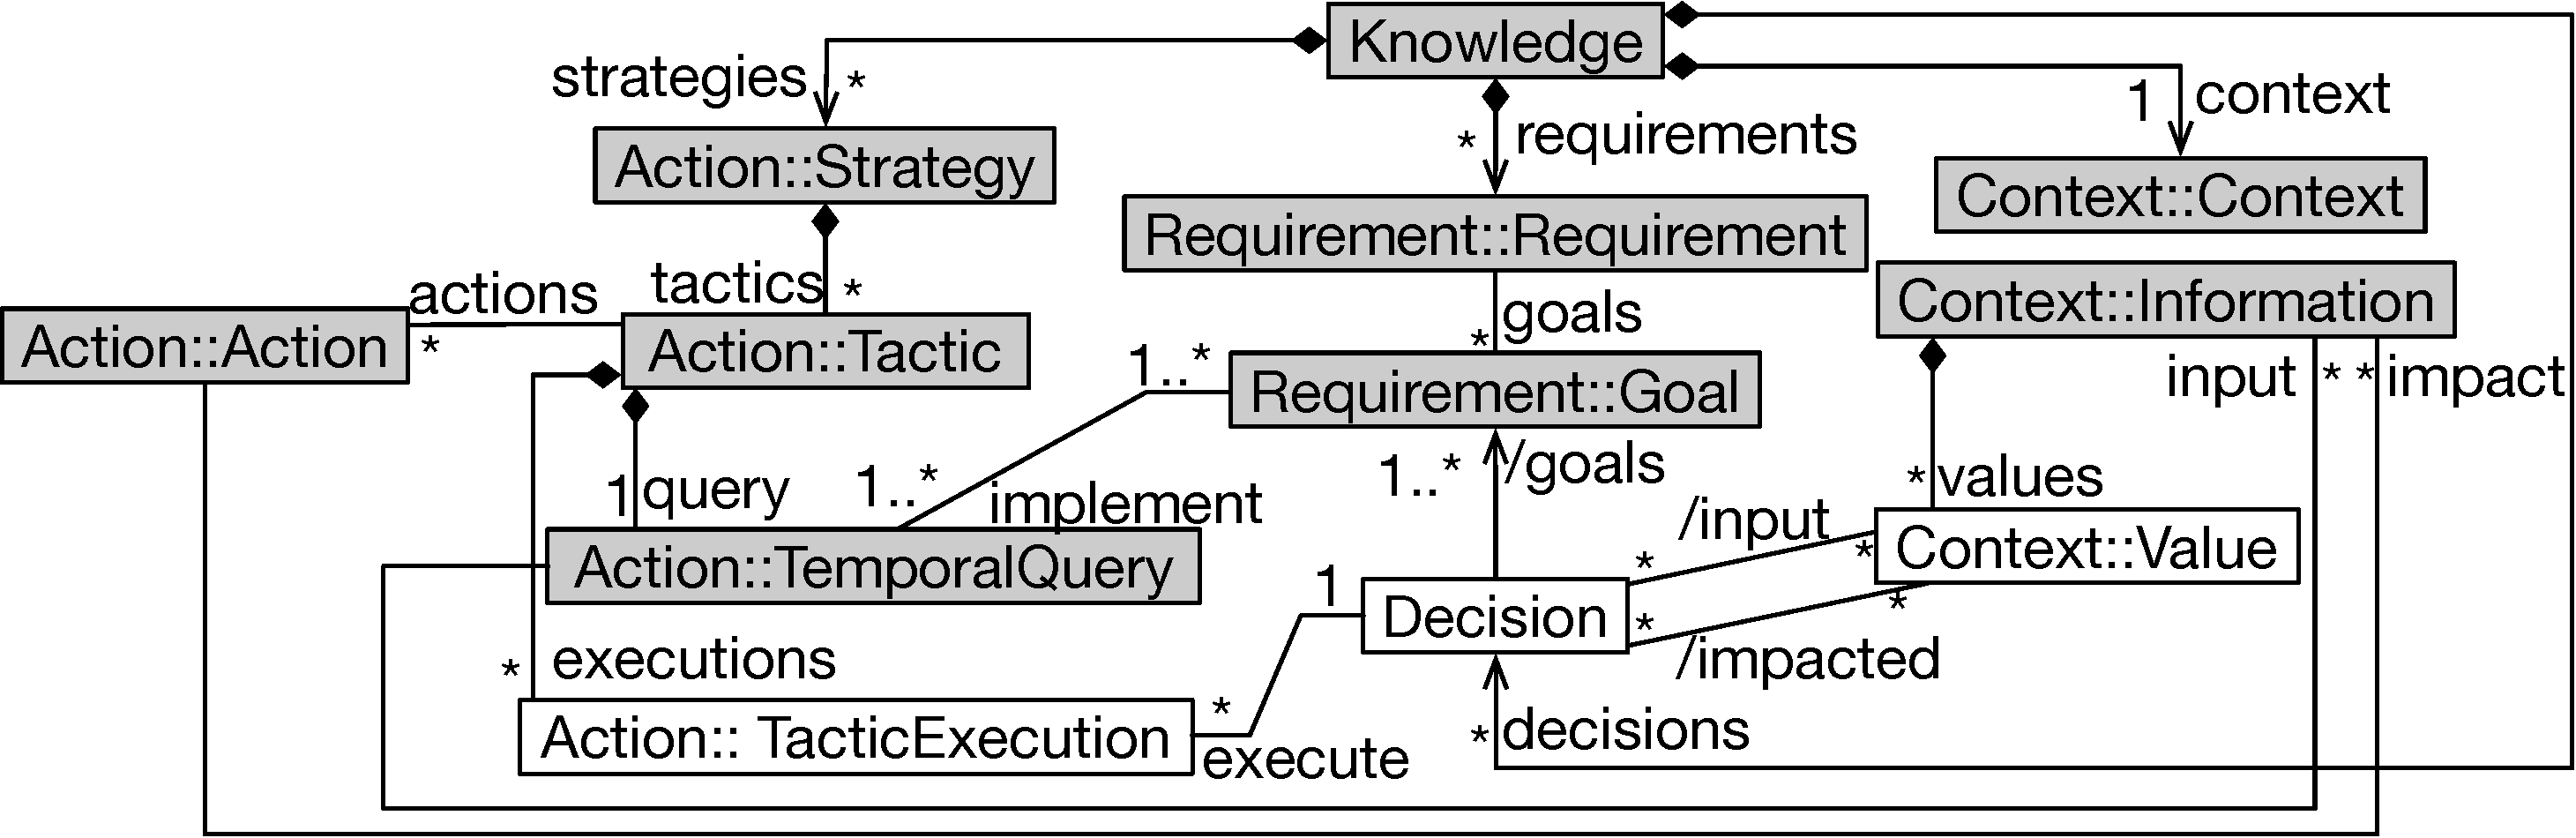
\includegraphics[width=.9\linewidth]{img/chapt-tkm/mm/knowledge-mm}
	\caption{Excerpt of the knowledge metamodel}
	\label{fig:knowledge-mm} 
\end{figure*}

In order to enable interactive diagnosis of adaptive systems, traceability links between the decisions made and their circumstances should be organized in a well-\linebreak structured representation. % todo still correct according to the global blabla
In what follows, we introduce how the \gls{knowledge} \gls{metamodel} helps to describe \glspl{decision}, which are linked to their  goals and their context (input and impact). 
Figure~\ref{fig:knowledge-mm} depicts this \gls{metamodel}.

Knowledge package is composed of a \textit{\gls{context}}, a set of \textit{\glspl{requirement}}, a set of \textit{strategies}, and a set of \textit{\glspl{decision}}.
A \gls{decision} can be seen as the output of the Analyze and Plan steps in the \gls{mapek} loop.

Decisions comprise target \textit{goals} and trigger the execution of one \textit{tactic} or more.  
A decision has an \textit{input} context and an \textit{impacted} context.
The context impacted by a decision  (\textit{Decision.impacted}) is a derived relationship computed by aggregating the impacts of all actions belonging to a decision (see Fig.~\ref{fig:action-mm}).
Likewise, the \textit{input} relationship is derived and can be computed similarly. 
In the smart grid example, a decision can be formulated (in plain English) as follows: since the district D is almost overloaded (\textit{input context}), we reduce the amps limit of greedy consumers using the ``\textit{reduce amps limit}" \textit{action} in order to reduce the load on the cable of the district (\textit{impact}) and satisfy the ``\textit{no overload}" policy (\textit{requirement}).

As all the elements inherit from the \textit{TimedElement}, we can capture the time at which a given decision and its subsequent actions were executed, and when their impact materialized, \ie measured.
Thanks to this metamodel representation, a developer can apprehend the possible causes behind malicious behaviours by navigating from the context values to the decisions that have impacted its value (\textit{Property.expected.impact}) and the goals it was trying to reach (\textit{Decision.goals}).
An example for such in interactive diagnosis can be found in Section~\ref{sec:tkm:intro:uc}.

\subsection{Context metamodel}
\begin{figure*}
 	 \centering
      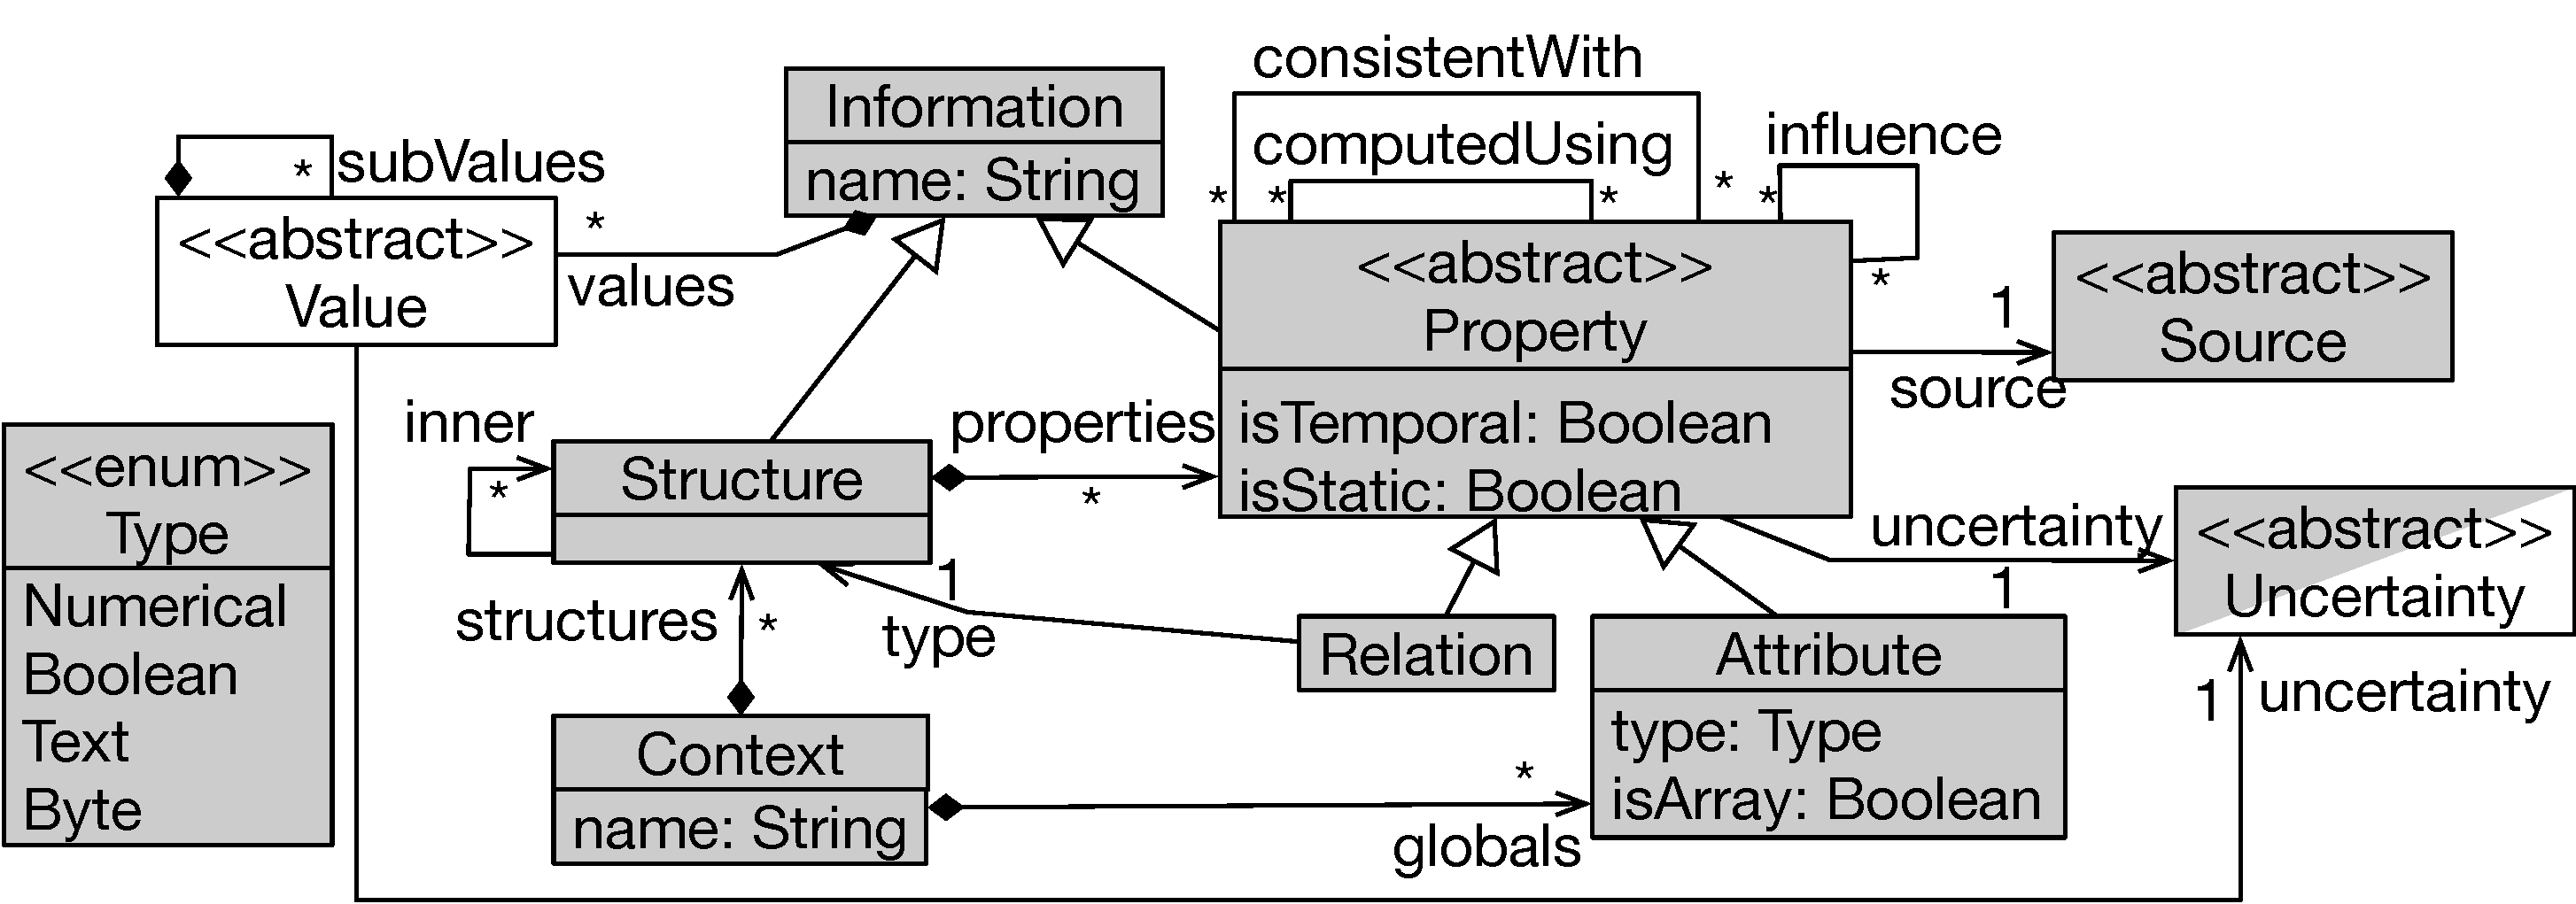
\includegraphics[width=.8\linewidth]{img/chapt-tkm/mm/contextModel}
      \caption{Excerpt of the context metamodel}
      \label{fig:context-model}
\end{figure*}

Context models structure context information acquired at runtime. 
For example, in a smart-grid system, the context model would contain information about smart-grid users (address, names, etc.) resource consumption, etc.

An excerpt of the context model is depicted in Figure~\ref{fig:context-model}. 
we propose to represent the context as a set of structures (\textit{Context.structures}) and global attributes (\textit{Context.globals}).
A structure can be viewed as a C-structure with a set of properties (\textit{Property}): attributes (\textit{Attribute}) or relationships (\textit{Relation}).
A structure may contain other nested structures (\textit{Structure.inner}).
Structures and properties have values.
They correspond to the nodes described in the formalization section (\cf Section~\ref{sec:tkm:k-formalism:formalism}).
The connection feature described in Section~\ref{sec:back:adapt:knowledge:req} is represented thanks to three recursive relationships on the Property class: \textit{consistentWith}, \textit{computedUsing} and \textit{influence}.
Additionally, each property has a source (\textit{Source}) and an uncertainty (\textit{Uncertainty}).
It is up to the stakeholder to extend data with the appropriate source: measured, computed, provided by a user, or by another system (\eg weather information coming from a public API).
Similarly, the uncertainty class can be extended to represent the different kinds of uncertainties. Finally, a property can be either historic or static.

\subsection{Requirement metamodel}

\begin{figure}
	\centering
	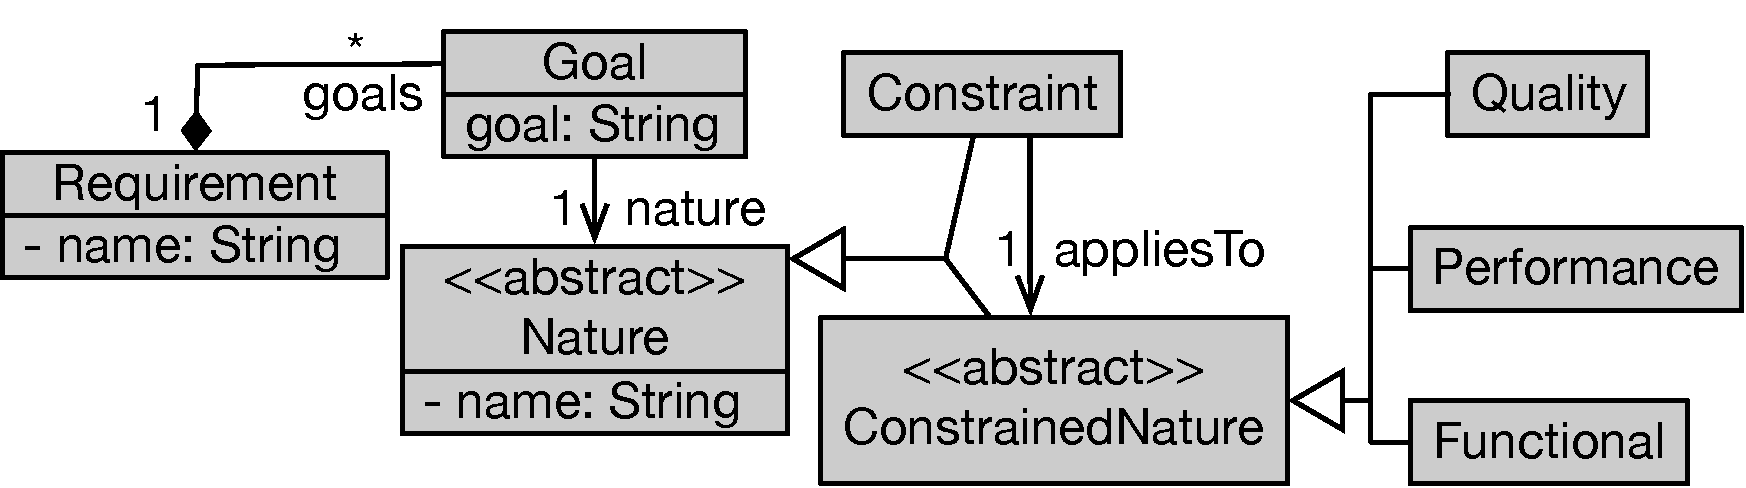
\includegraphics[width=0.7\linewidth]{img/chapt-tkm/mm/requirementModel}
	\caption{Requirement metamodel}
	\label{fig:requirement-model}
\end{figure}

As different solutions to model system requirements exist (\eg KAOS~\cite{DBLP:journals/scp/DardenneLF93}, i*~\cite{yu2011modelling} or Tropos~\cite{DBLP:journals/aamas/BrescianiPGGM04}), in this metamodel, we abstract their shared concepts.
The requirement model, depicted in Figure~\ref{fig:requirement-model}, represents the \textit{requirement} as a set of \textit{goals}.
Each goal has a \textit{nature} and a textual specification.
The nature of the goals adheres to the four categories of requirements presented in Section~\ref{sec:back:adapt:knowledge:req}.
One may use one of the existing requirements modelling languages (\eg RELAX) to define the semantics of the requirements. 
Since the requirement model is composed solely of design elements, we may rely on static analysis techniques to infer the requirement model from existing specifications.
The work of Egyed~\cite{DBLP:conf/icse/Egyed01} is one solution among others.
This work is out of the scope of the thesis and envisaged for future work. 

In the guidance example, the requirement model may contain a \textbf{balanced resource distribution} requirement.
It can be split into different goals: (i) \textit{minimizing overloads}, (ii) \textit{minimizing production lack}, (iii) \textit{minimizing production loss}.

\subsection{Action metamodel}

\begin{figure}
	\centering
	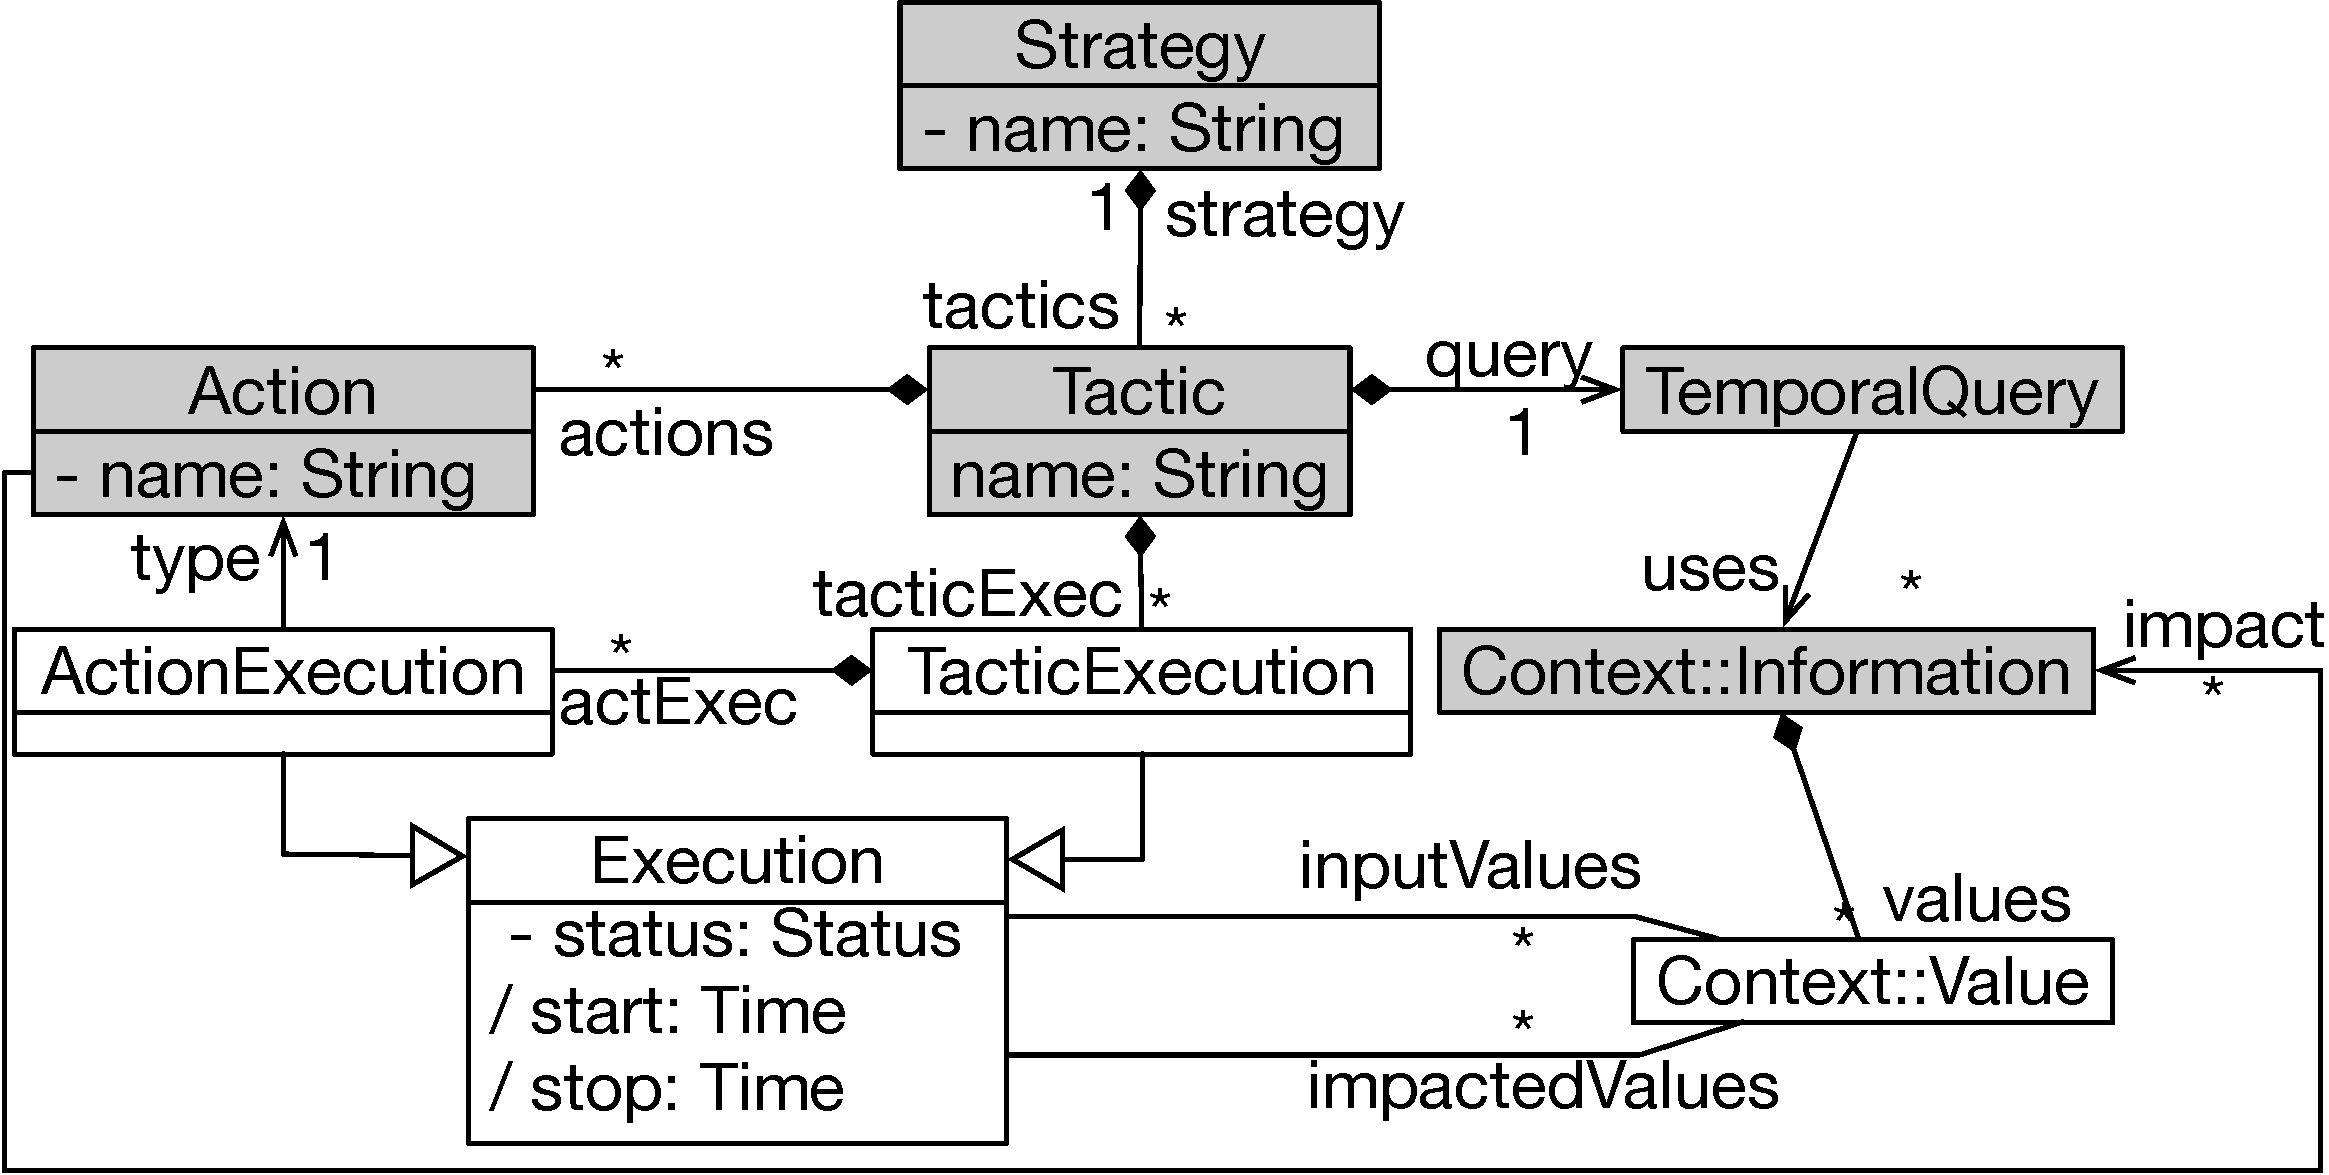
\includegraphics[width=0.8\linewidth]{img/chapt-tkm/mm/actionModel}
	\caption{Excerpt of the action metamodel}
	\label{fig:action-mm}
\end{figure}

Similar to the requirements metamodel, the actions metamodel also abstracts main concepts shared among existing solutions to describe adaptation processes and how they are linked to the context. 
Figure~\ref{fig:action-mm} depicts an excerpt of the action metamodel.
we define a strategy as a set of tactics (\textit{Strategy}).
A tactic contains a set of actions (\textit{Action}).
A tactic is executed under a precondition represented as a temporal query (\textit{TemporalQuery}) and uses different data from the context as input.
In future work, we will investigate the use of preconditions to schedule the executions order of the actions, similarly to existing formalisms such as Stitch~\cite{DBLP:journals/jss/ChengG12}.
The query can be as complex as needed and can navigate through the whole knowledge model.
Actions have impacts on certain properties, represented by the \textit{impacted} reference. 

The different executions are represented thanks to the \textit{Execution} class. Each execution has a status to track its progress and links to the impacted context values(\textit{Execution.impactedValues}).
Similarly, input values are represented thanks to the \textit{Execution.inputValues} relationship.
An execution has \textit{start} and \textit{end} time. Not to confuse with the \textit{startTime} and \textit{endTime} of the validity relation $V^T$.
Whilst the former corresponds to the time range in which a value is valid, the \textit{start} and \textit{stop} time in the class execution correspond to the time range in which an action or a tactic was being executed.
The start and stop attributes correspond to the relationL $E_{A_E}$ (see Section~\ref{sec:tkm:k-formalism:formalism}). These values can be derived based on the validity relation.
They correspond to the time range in which the status of the execution is \textquote{\textit{RUNNING}}.
Formally, for every execution node $e$, $E_{A_E}(e)~=~(V(e)~|~e.status~=~$\textquote{RUNNING}$)$.


Similarly to requirement models, it is possible to automatically infer design elements of action models by statically analyzing actions specification.
Since acquiring information about tactics and actions executions happens at runtime, one way to achieve this is by intercepting calls to actions executions and updating the appropriate action model elements accordingly.
This is out of the scope of this thesis and planned for future work.